
%% Add the 'procedia' option to approximate to the Word template
\documentclass[3p,procedia]{elsarticle}
\usepackage{ecrc}
\usepackage{color,soul}
\usepackage{multirow}
\usepackage{booktabs}
\graphicspath{{images/}}
\usepackage{lscape}
\usepackage{amssymb}
\usepackage{lineno}
\usepackage{hyperref}
\usepackage{subfig}
\usepackage[export]{adjustbox}
\usepackage{diagbox}

\usepackage{amsmath} 


\volume{}
\firstpage{1}
%\journalname{Forest ecology and management}
\runauth{}

\DeclareUnicodeCharacter{00E4}{\"a}% pour -niittyla

\begin{document}

\begin{frontmatter}

\author[label1]{Gilles Arthur}
\ead{arthur.gilles@uliege.be}
\author[label1]{Lisein Jonathan}
\author[label2]{Cansell Juliette}
\author[label1]{Latte Nicolas}
\author[label3]{Piedallu Christian}
\author[label1]{Claessens Hugues}

\fntext[label1]{Liège University - Faculty of Gembloux Agro-Bio Tech - unit of forest ressources managment}
\fntext[label2]{Centre National de la propriété forestière}
\fntext[label3]{Université de Lorraine, AgroParisTech, INRAE, Silva, 54000 Nancy, France}

\dochead{Original research papers}

\title{Evolution of the bark beetle crisis in the spruce forest: a remote sensing analysis in Belgium and North east France.}
\begin{abstract}
	
\iffalse




Following the droughts of 2018 to 2020, numerous Norway spruce diebacks were caused by bark beetles 
%(Ips typographus/ Pityogenes chalcographus)
outbreaks in Wallonia and in the Grand-Est. 
A methodology for detection the health status of spruce was developed based on satellite imagery from the European Union's Earth Observation Programme.
The time series of satellite images allowed the modelling of the spectral response of healthy spruce forests over the seasons. Deviations from this seasonal vegetation index trajectory for a healthy spruce stand are caused by a decrease in photosynthetic activity of the forest canopy.
This decrease in photosynthesis is caused by a bark beetle attack and is detected automatically.
This technique, inspired by the work of INRAe, is robust because of the redundancy of the information from the spatial images, which are repeated every 3-4 weeks. 
The method results in the production of annual maps of the health status of the Walloon and Grand-Est spruce forests.
The most important damage occurred in the years 2018-2019, affecting 2.8\% of the total area of spruce stands in Wallonia.

Although the main part of the crisis seems to be behind us, it remains to draw the necessary conclusions.
The relationship between climatic conditions and the presence of the bark beetle has proven to be complex in Wallonia.
Nevertheless, a very strong relationship between altitude and the presence of bark beetle damage could be demonstrated.
Stands below 300 m in altitude were indeed much more affected.
Moreover, forest sites located on steep slopes ( $\ge$  20 \%), whether on cold or warm slopes, are more affected than sites located on low slopes (plateaus).
In the Grand-Est, the peak of the crisis has been reached in 2019-2020. Altitude and slopes are not strongly influencing factors for spruce dieback. 

\fi
\end{abstract}

\begin{keyword}
  Norway spuce \sep Species vulnerability \sep Bark beetle \sep forest management \sep forest site \sep topographic condition \sep time series \sep Sentinel-2
\end{keyword}

\end{frontmatter}

%\linenumbers

\section{Introduction}

Global changes are increasing the risk of disturbances in forest environment: frequency and intensity of abiotic events (fire, storm, drought) and health problems (diseases and pest invasion) will be more recurrent \citep{lindner_climate_2010}.
In Western Europe, we expect a decrease of precipitation and an increase of drought events during the vegetation period, which will impact the actual geographic distribution of tree species \citep{hanewinkel2013climate}.
In this context, Norway spruce (\textit{Picea abies L. Karst}) which is one of the most important economic forest species in Europe \citep{nystedt_norway_2013} is also one of the most triggered species.
Indeed, this species is very sensitive to water shortage \citep{tjoelker_outline_2007} and lack of water induces stress that affect growth and health of the tree.
Moreover, its major pest, the bark beetle, causes important outbreaks after storm, which provide breeding material e.g. windfalls, or after severe drought that weaken trees.
A recent bark beetle crisis, triggered by the exceptionally hot and dry weather of 2018, occurred in Western Europe. 
It has highlighted the need of improving our understanding of both Norway spruce and bark beetle autecology and synecology for minimizing the impact of bark beetle on spruce stands with adapted management methods.
It should concern the monitoring of bark beetle population and early detection of attacks on trees as well as adapted silvicultural methods and adequate species composition of future forest, especially in the thousands of clear-cutted hectares decimated by bark beetle attacks. 
The Norway spruce is a native species of the boreal or mountainous climates of Europe.
It is naturally present in the highest altitude in the Vosges mountains, but it has also been successfully planted out of its native range on warmer sites of low altitude in the Grand-Est (France) and Wallonia (Belgium) during the $19^{th}$ and $20^{th}$ centuries \citep{Noirfalise_1975,guinier_trois_1959}.
The massive reforestations occurring at this time have led to the formation of large pure even-aged stands.
It usually develops a taproot system with fine roots in shallow depth, although rooting system can adapt its configuration in constrained soil conditions \citep{puhe_roots_2003,kostler_1968}.    
Stressed Norway spruce produce volatile compounds which attract bark beetles, making himself more susceptible to pest attack \citep{netherer_waterlimiting_2015,netherer_interactions_2021}.
Bark beetles, in particular the species \textit{Ips typographus}, are ubiquitous in the forest and their populations are generally low (endemic phase) without producing damage to healthy trees. 
However a large amount of stressed trees causes a shift to an epidemic phasis with a explosion of bark beetle populations during which even healthy trees are massively attacked \citep{kautz_individual_2014}.
The life cycle of bark beetle depends on temperature and photoperiod \citep{annila_influence_1969, baier_phenipscomprehensive_2007}.
In Northern Europe, the bark beetle is univoltine (one single generation) but it is multivoltine (breed two or even three generations) in Western and Central Europe \citep{annila_influence_1969}.
After spring swarming, the adult enter in the bark and burrow wood to make brood gallery where they mate and lay the eggs that mature to larvae into the phloem \citep{hlasny_bark_2021}.
The bark beetle adult can re-emerge and swarm a second time to give birth to one sister brood \citep{zolubas_1995}.
After the larvae maturation that last about seven weeks \citep{baier_phenipscomprehensive_2007}, the new generation of beetles emerges and attacks the direct surrounding trees \citep{zolubas_1995}.
Attacked trees defend themselves by pulsing resin to kill the bark beetle but these defence failed to resist again numerous simultaneous attacks that induce their decline and rapid death.
The Norway spruce dieback goes through three physiological stages which are denominated green, red and grey stage.
During the green stage, the bark beetle has succeeded to penetrate the phloem and the spruce retains its green needles. 
The tree is still alive but begins to suffer of water shortage caused by sap conduction problem. 
After several weeks, the red stage is reached when the needles turn brown-red. The tree is recently dead and the dry needles start to fall.
When all the needles of the spruce have fallen off and the grey bark of the trunk is visible, the grey stage is reached \citep{abdullah_european_2018}. 
To control the infestation of bark beetle, the practical solutions are limited. 
The use of phytosanitary product is forbidden in Belgian and French forest.
Pheromone trap systems are commercialized to fight bark beetle but they failed to limit the economic loss in case of large outbreak \citep{kuhn_pheromone_2022}.
The only solution to limit the bark beetle population and its associated damages is to fell and remove each attacked tree at the green stage, before the swarming.
It takes this ideal breeding material out of the forest.

The European Union’s earth observation program, with its satellite twin constellation Sentinel-2A and Sentinel-2B, provides free earth imagery with a high revisit time, which have been intensively used for forestry purpose. 
Time series of Sentinel-2 (S2) images enable to model the phenology courses of vegetation indices in order to detect forest disturbances \citep{low_phenology_2020}, like the one caused by bark beetle outbreaks.
Infestation maps of the last sanitary crisis have been generated for Germany \citep{ali_canopy_2021,thonfeld_first_2022}, Czech Republic \citep{barta_early_2021}, Italy \citep{dalponte_mapping_2022} and France \citep{nardi_drought_2022}. 
This paper aims to assess the evolution of the bark beetle crisis during the 2017-2022 period in the Walloon and Grand-Est spruce forest using remote sensing.
To this end, we map Norway spruce dieback using S2 time series.
Then, we analyse the relationship between the level of bark beetle damages and some main environmental parameters such as altitude and topography in order to determine the most sensitive forest sites where Norway spruce forestry should no longer be considered.

\section{Material and methods}
\subsection{Study area}

The study area include Wallonia (south of Belgium) and the Grand-Est region (north-east of France).
The Walloon forest covers 554,600 ha and  Norway spruce stands occupy quarter of area \citep{lejeune_ep_2022}.  
The Norway spruce covers seven percent of the 1,939,000 ha of the Grand-Est forest \citep{IGN2022}. 
Both neighbour countries share some similar environmental conditions.
They are included in the temperate oceanic bioclimatic zone \citep{lindner_climate_2010}.
However at a finest scale, 24 ecoregions have been defined in  Wallonia and Grand-Est, mainly by climate and soil parameters and therefore influence the tree species distribution \citep{walthert_tree_2017}.
To better analyse the dieback of Norway spruce, the French and Walloon ecoregions have been grouped in three main regions according to average temperature and precipitation during the growing season (May to September) of the 1991-2020 period in three homogeneous bioclimatic areas: Plains, Ardenne and Vosges (Figure \ref{fig:clim}).
Plains are characterized by the lowest rainfall during the growing season ($<$ 400 mm) and among the highest mean temperature during the growing season ($>$ 15 °C).
Ecoregions with rainfall between 400 mm and 450 mm and temperature lower than 15.5°C correspond to the bioclimatic area of the Ardenne.
Vosges are ecoregions with the highest rainfall ($>$ 400 mm) and temperature between 15.5 °C and 17°C.
The climate variables for Wallonia have been provided by the Royal Meteorological Institute of Belgium and come from the climate maps Digitalis for the Grand-Est \citep{piedallu_presentation_2014}.
These three regions differ in their altitude which can be considered as an imperfect proxy for climate (Figure \ref{fig:situ}). 
The altitude varies between 100 m and 500 m for the Plains, between 200 m and 700 m for the Ardenne and between 300 m and 1500 m for the Vosges.
The majority of spruce in the Plains is located in low altitude under 300 m in contrast with the Ardenne and the Vosges where the majority of Norway spruce stand grow above 400 m. 
The studied spruce area covers 107,926 ha in Ardenne, 75,067 ha in the Vosges and  24,462 ha in the Plains.% in the Grand-Est region.

\begin{figure}[htbp] 
	\centering
	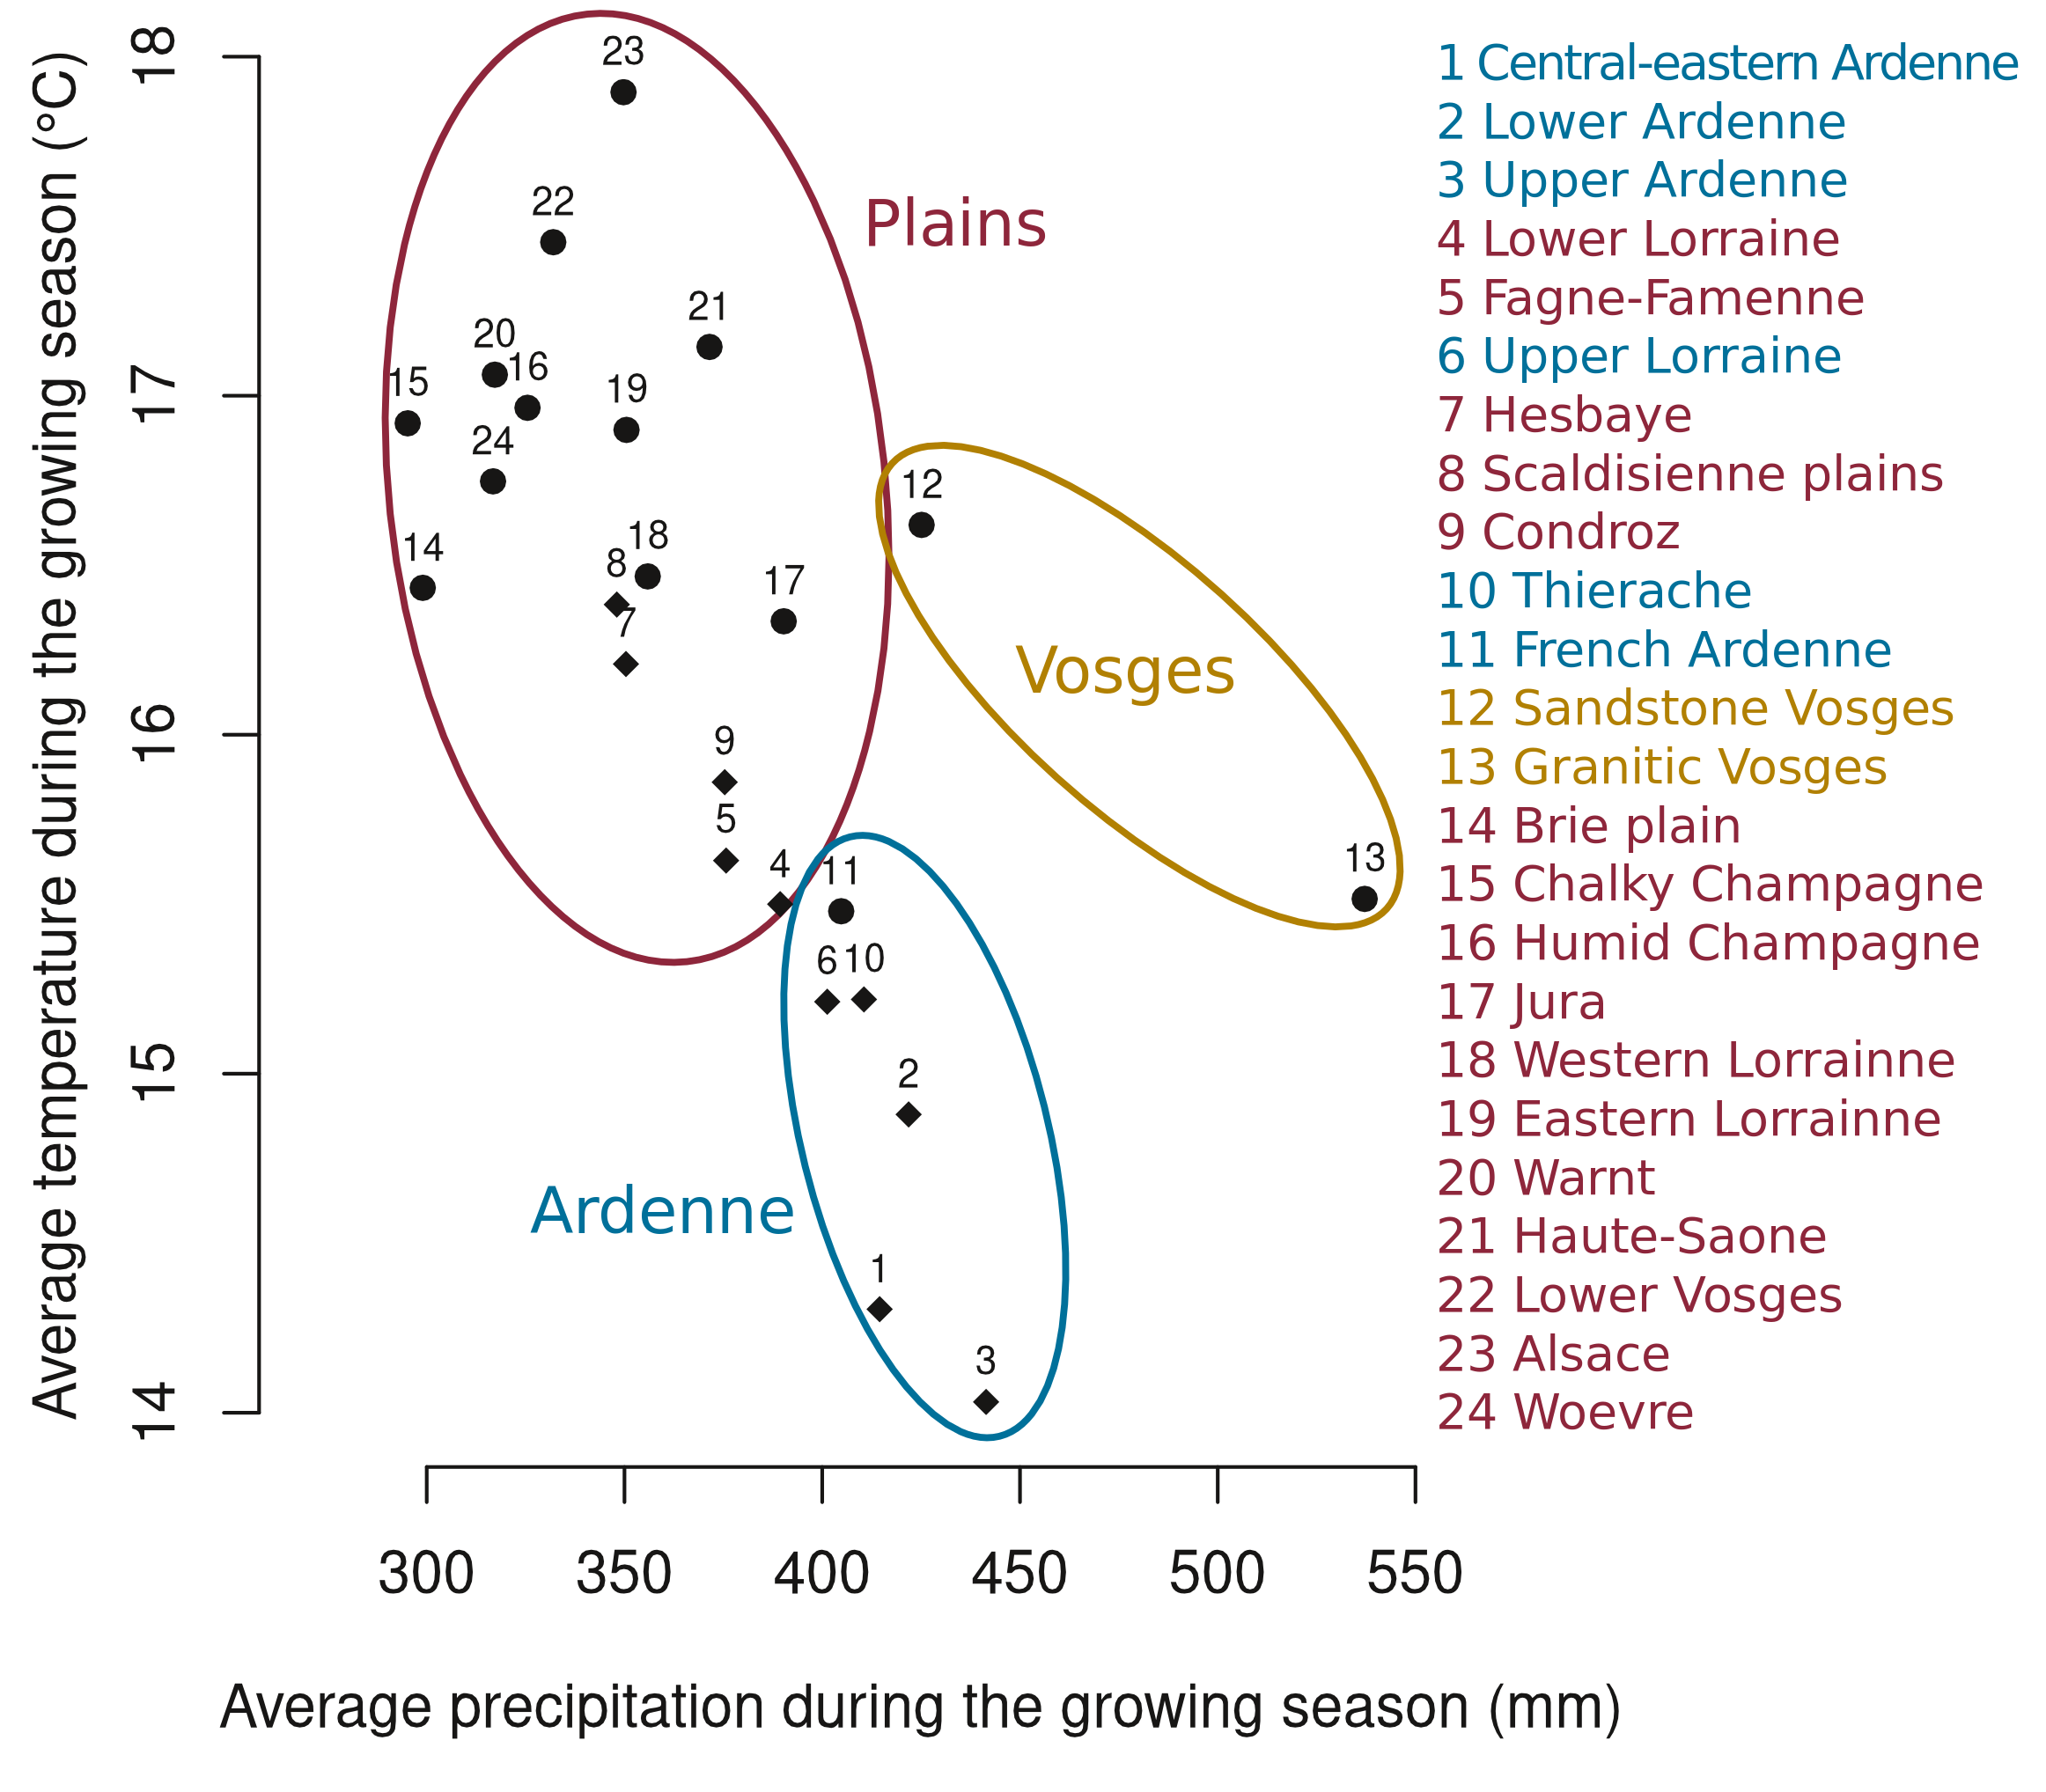
\includegraphics[width=0.8\linewidth]{climat/climat_region.png}
	\caption{Groups of ecoregions according to the temperature and precipitation of the growing season (may-septembre) during the 1991-2020 period: Ardenne (blue), Plains (red) and Vosges (orange). Walloon ecoregions are depicted with cross, and Grand-Est regions are illustrated by rounded points.}
	\label{fig:clim}
\end{figure}

The regional climate is locally influenced by topography \citep{de_frenne_forest_2021}.
South-facing slopes are warmer and drier and their temperature difference between day and night are greater than the North-facing ones.
Three topographic exposures have been determined using the \cite{Delvaux_galoux} definition.
Plateaus and plains are neutral topographic conditions and valley floor that does not create a particular local climate.
Comparatively to flat areas, north-facing orientations are slopes greater than  20\% facing north (285° to 125°) with colder and more shades conditions.
South-facing orientations are slopes greater than  20\% facing south (125° to 285°) with a warmer local climate.
The digital elevation model (DEM) data from the Copernicus Land Monitoring Service \citep{DEM_copernicus} at a resolution of 25 m have been used for altitude and topographic exposures maps.

\begin{figure} [htbp] 
	\centering
	\includegraphics[width=0.8\textwidth]{ze_v_uk.png}
	\caption{Study area: Plains (hashed, altitude varying between 100 and 500 meters above see level), Ardenne (black dot, altitude between 200 and 700 m) and Vosges (cross, altitude ranging from 300 to 1500 m). Red squares illustrates the extend of Sentinel-2 tiles which are used for the detection of bark beetle attack. The centroid of each ecoregion is represented by purple dot.}
	\label{fig:situ}
\end{figure}

\subsection{Mapping of healthy and dieback spruce stands}
The first prerequisite to assess spruce dieback was to map the species distribution at a fine scale.
For the south of Belgium, we used reliable composition maps from \cite{bolyn_mapping_2022}, computed from remote sensing data, in order to restrict our analysis to Norway spruces. 
These composition maps consist in presence probabilities for eight major species, from which we discriminated Norway spruce stands by selecting areas with equals or greater than 80\% of probability of presence for this species.  
In the Grand-Est, the composition map came from the French national geographic agency \citep{IGN_bd_2018} and forest stand composition was determined by photointerpretation.
We first selected forest stands identified as \textit{spruce or fir} in order to restrict the dieback analysis. 
Phenology courses are highly suitable for forest tree species discrimination \citep{lisein_discrimination_2015,grabska_forest_2019,ma_tree_2021}.
Sentinel-2 (S2) spectral bands courses along the vegetation season were used to refine the determination of species present in the area interpreted as \textit{spruce or fir} in the Grand-Est. 
S2 satellites carry multispectral sensor with a ground resolution up to 10 m. 
Bottom of Atmosphere reflectance images (L2A product) were downloaded from the Theia data cluster \citep{theia_team} for all the 14 tiles of 100km x 100km covering our study area (Figure \ref{fig:situ}), provided that the cloud cover does not exceed 35 percent.
In order to identify and remove every pixel that did not correspond to spruce stand in the Grand-Est, all S2 spectral bands of 10 and 20 meters ground sample distance were first summarized for each of the four quarters of the year, by averaging all cloud-free observations occurring during the quarter.
We used the satellite observations from the two years prior to the bark beetle crisis for computing these multi-year quarterly averages, i.e. 2016 and 2017.
A Random Forest algorithm was then trained on this synthetic time serie to discriminate spruce from non-spruce pixels, based on a training set of observations from Belgium consisting in 1000 sampled pixels (20mx20m) for each of the eight major species \citep{bolyn_forest_2018}.
This forest species classifier was applied on \textit{spruce or fir} area of Grand-Est. 
The proportion of pixel detected as spruce in the \textit{spruce or fir} stands of the Vosges was 67 \% and correspond to the level of mixture expected for this bioclimatic area.  
Following bark beetle detection was carried on only for 10x10 m pixels detected as spruce.

The detection of Norway spruce dieback was realized by using dense time series of S2 imagery following the methodology developed by \cite{dutrieux_package_2021}.
Vegetation changes were tracked by means of a phenology metric, the \textit{SWIR Continuum Removal} vegetation index ($SWIR_{CR}$).
The $SWIR_{CR}$ is based on three spectral bands, the near-infrared, the shortwave infrared 1 band and the shortwave infrared 2, and is sensitive to the foliage water content: it is theoretically appropriated to detect spruce dieback during the green stage of bark beetle attack (Figure \ref{fig:harmo}).
Seasonal variation of $SWIR_{CR}$ for healthy stands was modelled by fitting an harmonic function on 300 spruce pixels interpreted as healthy on orthophotoplan. 
The harmonic function is presented in equation \ref{eq:harmo} where $t$ express the time as being the day of the year.
\begin{equation}\label{eq:harmo}
SWIR_{CR}(t) =   a_{1} + b_{1} \sin(\dfrac{2\pi}{365.25}t)+ b_{2} \cos(\dfrac{2\pi}{365.25}t)+ b_{3} \sin(\dfrac{2\pi}{365.25}2t)+ b_{4} \cos(\dfrac{2\pi}{365.25}2t)
\end{equation} 
For fitting this equation on the 300 healthy spruce pixels, we used all cloud-free S2 observations from the two years preceding the onset of the bark beetle crisis, i.e. 2016 and 2017.
Then, bark beetle attack was detected if the $SWIR_{CR}$ observations deviate from the healthy phenology trajectory. 
Preliminary investigations have led us to consider a multiplying factor of 1.7 applied to the $SWIR_{CR}$ for determining the threshold separating healthy to stressed situation.
Figure \ref{fig:harmo} illustrates a time serie of $SWIR_{CR}$ observations (grey dots) for one single pixel. 
When the observations exceed the threshold represented by the purple-dashed line (in 2019 in Figure \ref{fig:harmo}), the spruce stand is probably under severe stress.
As soon as $SWIR_{CR}$ vegetation index showed a stress for two consecutive times separated by at least 20 days, we assumed that the stress is permanent and made sure that this pixel cannot return to a healthy situation in the following observations.
In parrallel to the detection of bark beetle stress, stand cutting and thinning were subject of particular attention: 
bare soil was detected by using a combination of thresholds for red, green, blue and shortwave infrared reflectance values (Band 8A $\geq$ 12\% reflectance and Band 2 $\leq$ 6 \% reflectance and Band 3 + Band 4 $\geq$ 8 \% reflectance).
Cutting were thus taken into account and were classified either as normal harvest cutting or as sanitary thinning based on the health status determined by the $SWIR_{CR}$ vegetation index prior to the cutting.
Although \cite{dutrieux_package_2021} have published their methodology as a open-source python package, named \textit{FORDEAD}, we have adapted the pipeline in C++ in order to comply with our specific requirements.
Our code is online on github repository (\url{https://github.com/JoLeBelge/s2-spruce-dieback/}). 
We made use of OTB toolbox \citep{grizonnet_2017_OTB} for image processing and the health status was summarized by annual health maps in raster format.
The annual health maps cover the period starting from may and finishing in april of the next calendar year, because we made the assumption that Norway spruce dieback detected in april are related to bark beetle attack from the previous calendar year \citep{muller_features_2022}.
This analysis of image time serie was performed on S2 observations between first may 2017 and 28 february 2023 and the health status of every single pixel (10 meters resolution) located in a spruce stand was classified in one of the four following classes ; healthy, bark beetle attacked, cutted or sanitary thinning.
This comprehensive time serie of almost six years counted a minimum of 134 and maximum 275 acquisition dates according to the location and totalized a volume of 5.0 Tbit with intermediate results.
For every single vegetation year, we enumerated a minimum of 10 and maximum of 65 acquisition dates (median = 30), always with a cloud cover smaller than 35 \%.
A post-processing of the spruce health maps was finally carried out in order to take into account certain neighborhood relationships. 
Area of cutted spruce directly surrounded by areas classified as sanitary cutting where detected and were considered also beeing part of the sanitation felling if the number of neighbouring dieback pixels (8-neighbours relationship) exceed 50 \% of the number of pixel composing the cutted spruce area.

\begin{figure}[htbp] 
	\centering
	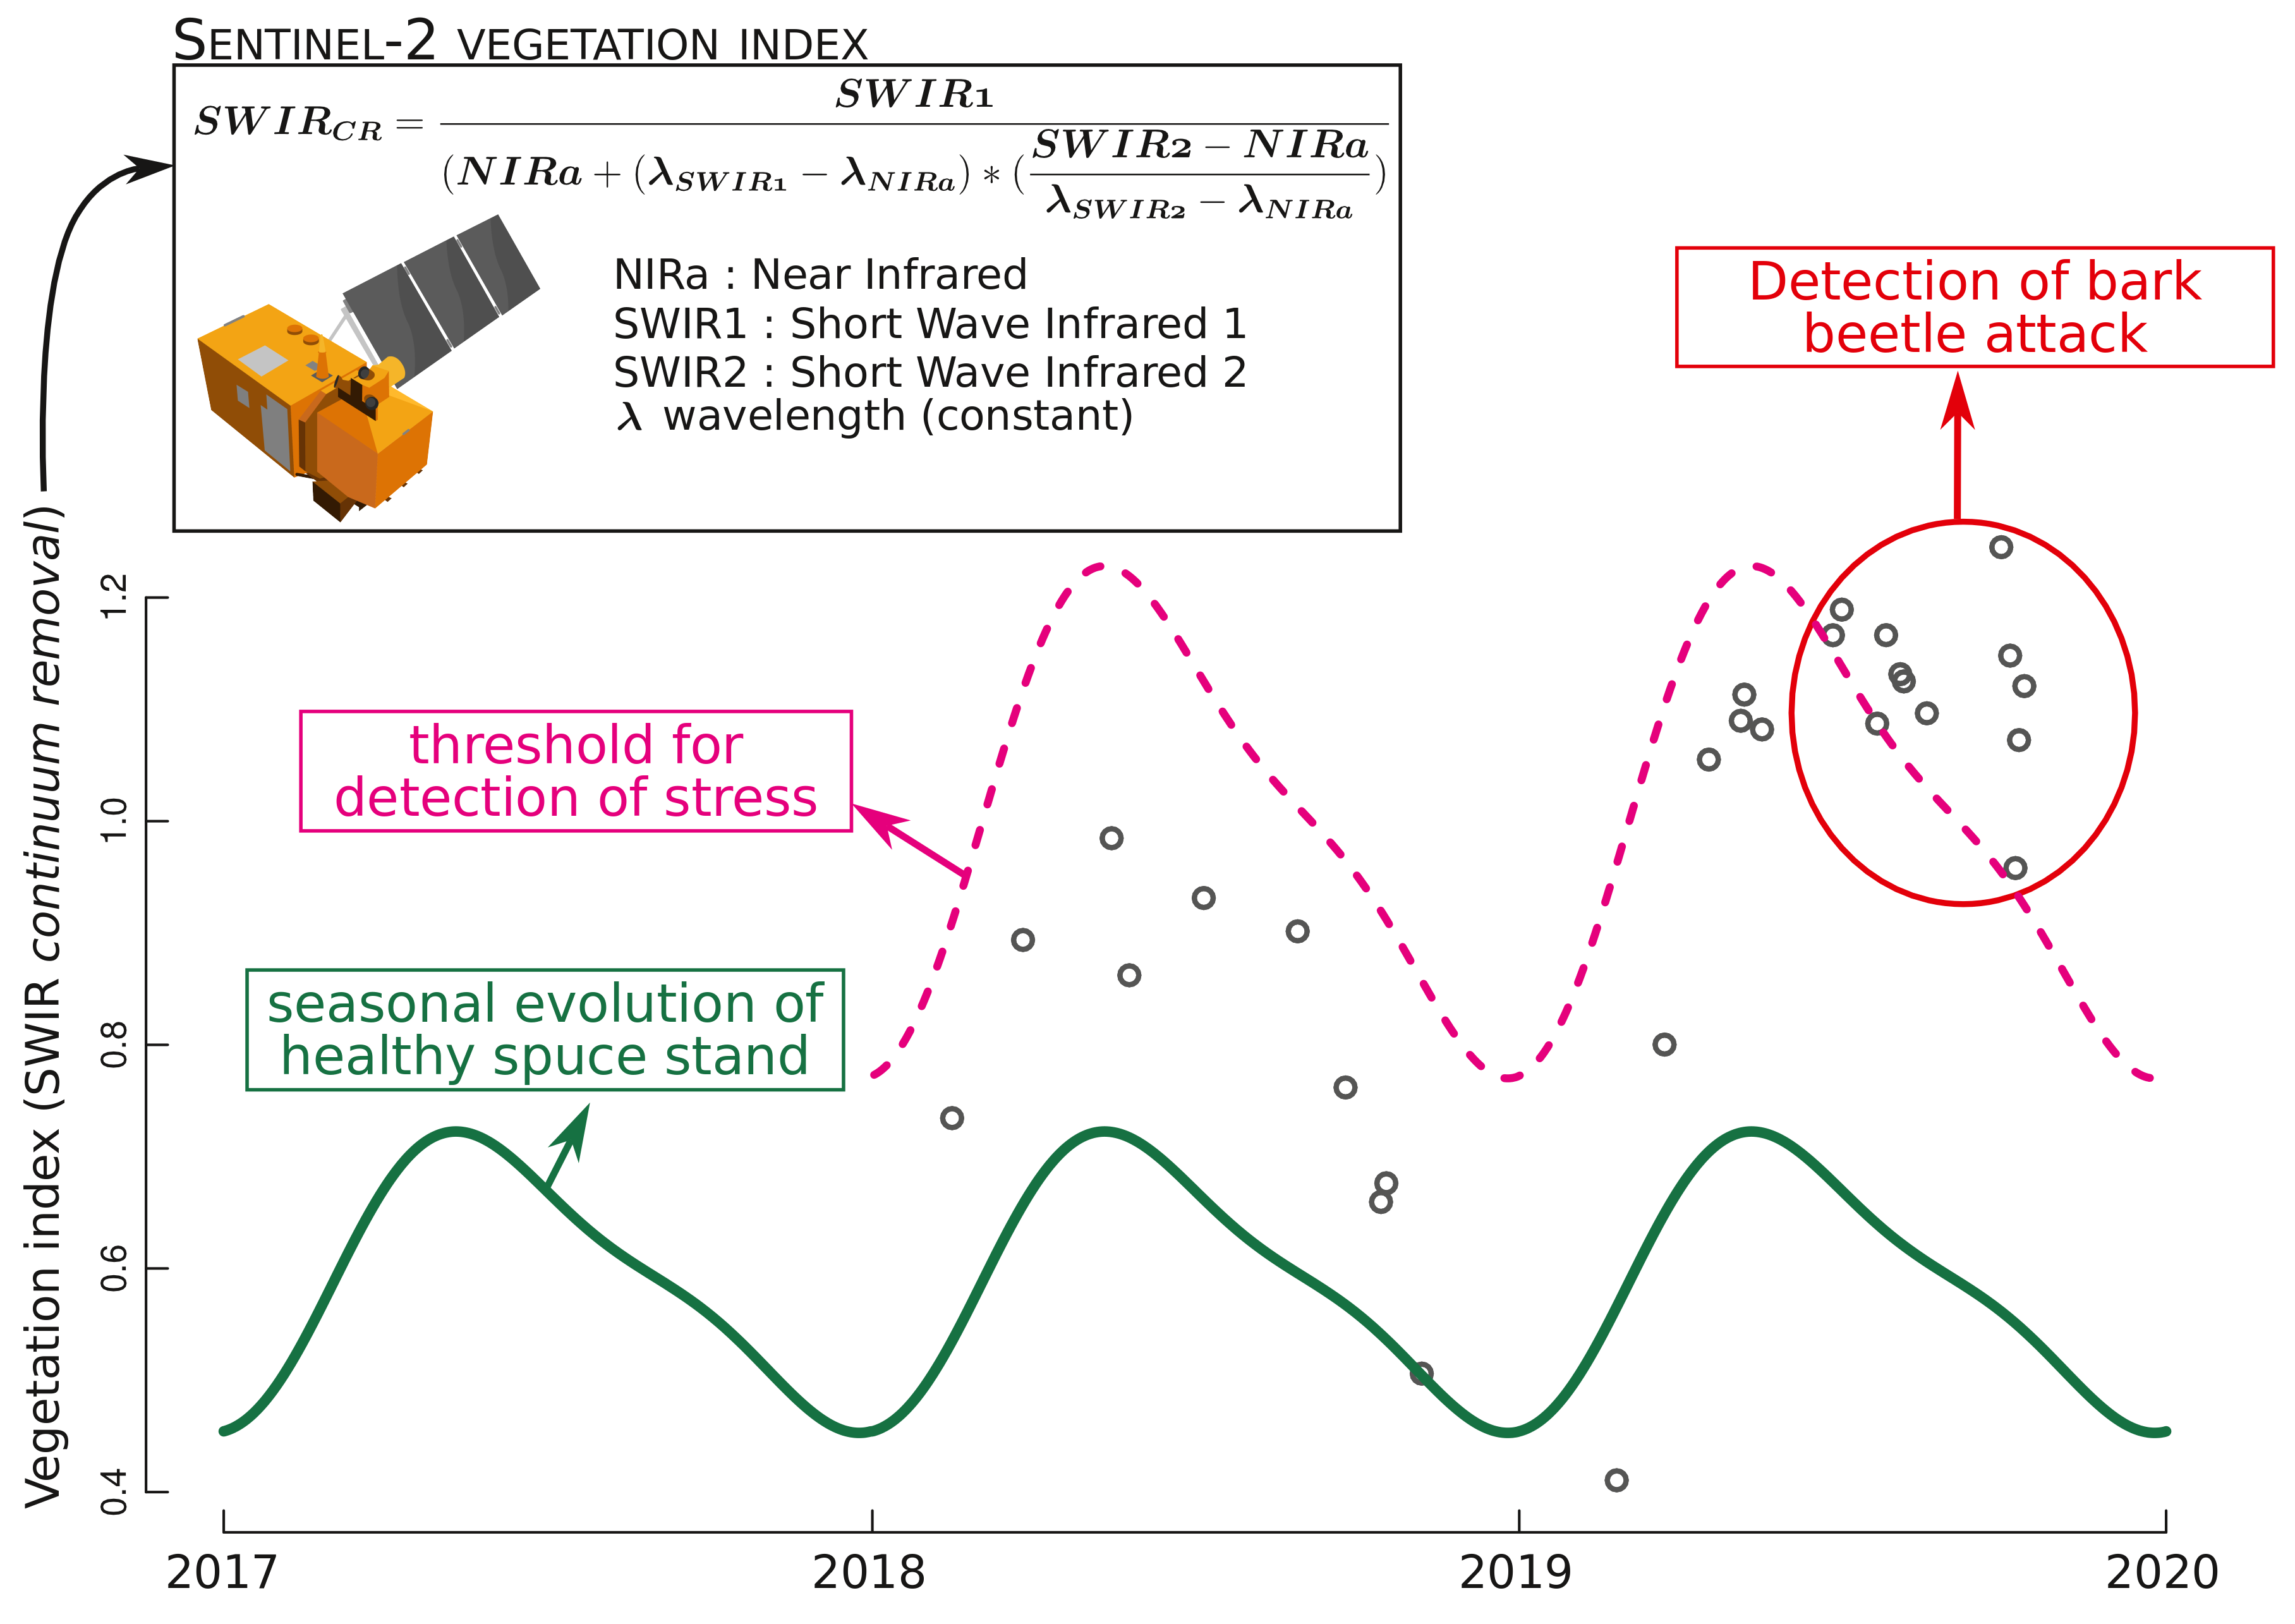
\includegraphics[width=0.8\textwidth]{fctHarmo.png}
	\caption{Bark beetle health maps were computed by detecting change in the $SWIR_{CR}$ phenology metric. The \textit{SWIR Continuum Removal} was computed using three bands from Sentinel-2 imagery for every single acquisition date and its value was compared to a threshold (purple dashed line, which correspond to the healthy situation in green multiplied by 1.7) in order to detect vegetation stress. If a stress was detected two consecutive times with a minimum of 20 days between the observations, we assumed that the dieback occurred.}
	\label{fig:harmo}
\end{figure}

The spruce health maps were validated by two different methods.
On the one hand, a stratified random sampling based on the size of the dieback area on the spruce health map was used for the 2018 vegetation season.
The dieback area is a combination of bark beetle attacked area and sanitary cutting area.
Adjacent pixels of dieback were first gathered, polygonized and categorized into six surface categories ; $\leq$ 200 m²,  200 $<$ and $\leq$ 400 m², 400 $<$ and $\leq$ 600 m², 600 $<$ and $\leq$ 1000 m², 1000 $<$ and $\leq$ 2000 m² and eventually $\geq$ 2000 m².
We selected 48 dieback polygons for each surface categorie (total of 288) located exclusively in Belgian Ardenne and we performed a photointerpretation with the annual orthophotoplans of the Wallonia. 
The sanitary status from the health map was compared with health status deduced from the orthophotoplan and false detection were expressed as the proportion of surface wrongly detected as dieback.
This validation focused only on dieback observations and did not take into account healthy observations as its objective was to quantify the proportion of false detection, i.e. areas falsely detected as dieback by the time series analysis.
On the other hand, a field validation in the Vosges massif was carried out on 95 stands between february and april 2021.
The selection of the circular field plots (diameter of 30 meters) was made on the basis of the photo-interpretation of the annual orthophotoplan in order to balance the number of healthy and dieback plots. 
Each stand have been inspected for the presence of bark beetles or dead trees and this health status have been compared with the spruce health map. 

\subsection{Relation between bark beetle attack and topographical conditions}

The forest practitioners of the two countries drew our attention to the variables that seemed to influence spruce dieback.
According to them, the south-facing slopes and low altitude favor the spruce dieback.
This hypothesis match with autecology of spruce, that is known to suffer from heatwaves and low water availability.
Indeed, in the study area, precipitation increase with altitude, temperatures decrease the higher the altitude at least within the tree main ecoregions.
In addition, the warmer climate of south-facing slopes favours the development of bark beetle population \citep{annila_influence_1969, baier_phenipscomprehensive_2007, jonsson_2009, marini_climate_2012} and increase the susceptibility of Norway spruce to the attack of bark beetle \citep{wermelinger_ecology_2004, netherer_waterlimiting_2015}.
Following this theory, there should be more attacked Norway spruce in low altitude and in south-facing slope in the three climatic areas.  
Sanitary map has been used to study the relation between the dieback and these two topographic variables.
%climat proxi altitude 
%altitude facile à avoir sur deux pays à haute resolution
%Microclimat ss 
% basse altitude % Sous secteur chaud  + plus chaud - de pluies don cfavorable aux scolyte et defavorable àl'épicéa
% Sous secteur chaud 
The altitude has been broken down  by 100 m classes and kept the three topographic exposures classes.
To determine which class of the two topographic variables was most affected, we estimated the dieback areas for each class of each factor based on the health status maps for each year of the period 2017-2021.
The  annual dieback rate is  the dieback area of a class during one year divided by the total area of Norway spruce of this class at the beginning of the same year. 
Dieback area is the surface of Norway spruce attacked by bark beetle and the area of sanitary cutting during the year. 
The total area of spruce at the beginning of the years is composed of the area of healthy spruce area at the beginning of the year. 


%mettre equation 
%\[
%\frac{\sum dead\, spruce\, area\, of\, the\, year }{\sum spruce\, area\, at\, the\, beginning\, of\, the\, year\,}\]



  
			
% Classe d'latitude
%calcul prob prese
%Comparaison entre le différents pays
%Depuis 2018, des attaques massives de scolytes tuant les épicéas frappent la Wallonie. Suite à ces évenements,les forestiers se sont interrogés sur cerains facteurs topographiques semblant avoir fortement influencé les attaques de scolytes.
%Les pessières situées en basse altitude semblent avoir été plus touché ainsi que les peuplement situé sur des versants sud.

%Pour caracteriser les attaques de scolytes, nous avons appliquer la méthode des random forest afin de selectionner les 2 facteurs topographiques influençant le plus les attaques de scolytes. CEs deux facteur sont l'altitude et les sous-radiatif. Nous avons ventilé l'altitude par classe de 100m et conservé les trois classes de sous secteurs définis par delvaux et galoux.

%Ensuite, afin de determiner les classes de ces facteurs les plus impactés par le scolyte, nous avons estimé les surfaces scolytés pour chacune des classes de chaque facteurs sur base des cartes d'état sanitaire pour chaque année de la période 2016-2021.

%La carte d'etat sanitaire de la pessière a été subdivisée en tuile de 50*50m (25 pixel de 10X10m) comprenant au minimum 17 pixel de 10mX10m d'épicéas. Une tuile est considérée comme %scolytée quand minimum 3 pixels sur 25 sont scolytés.

%Pour chaque tuile, la classe d'altitude et le sous-secteur ont été extraits.

%Nous avons calculé le ratio du nombre tuiles scolyté d'une classe divisé par le nombre total de tuiles de la classe (probabilité de présence) pour chacune des classes d'altitude et de sous-secteurs.


%\begin{align*}

%$presence\,of\,probability = \frac{tiles\, affected\, by\, the\, bark\, beetle\, of\, a\, class}{total\, number\, of\, tiles\, in\, the\, class}$

%\end{align*}



%However, other factors such as degres day data could influence bark beetle attacks 
%We made a selection of factors influencing bark beetles favourably and norway spruce unfavourably using the random forest method. The factors emerging from this analysis show that altitude and radiative topography orientation are the most important factors 






\section{Results}


\subsection{Sanitary map validation}
The photo-interpretation of spruce stand crossed with the sanitary map shows when the sanitary map predicts a decline, the dieback is confirmed by the orthophotoplan in 86.1 \% (table \ref{tab_confu_matrix}) of the verified spots.
In 13.9 \% this is a false positive because the trees are still healthy.
  
\begin{table}[htbp] 
\caption{Sanitary map validation using aerial photographs for 274 spruce stands.}
\label{tab_confu_matrix}
\begin{tabular}{|l|l|l|}
\hline
\diagbox{Sanitary map}{Orthophotoplan} & Dead trees & Healthy trees \\ \hline
Attacked trees                    & 86.1 \%   & 13.9 \%      \\ \hline
\end{tabular}
\end{table}

The field validation in the Vosges confirms the result of the photo-interpretation method.
Dead stand are identified correctly in 84.7 \%.
The healthy stands on the sanitary map are valided in 100 \% of the stand  in the field (Table \ref{field_confu_matrix}).
\begin{table}[htbp] 
\caption{Sanitary map validation for 95 spruce stands using field survey in the Vosges mountains.}
\label{field_confu_matrix}
\begin{tabular}{|l|l|l|}
\hline
\diagbox{Sanitary map}{Field} & Dead trees & Healthy trees \\ \hline
Dieback trees (=39)                    & 84.7 \%  & 15.3\%      \\ \hline
Healthy trees (n=56)                    & 0 \%      & 100 \%
\\ \hline
\end{tabular}
\end{table}



\subsection{Evolution of the crisis}

After a low spruce mortality rate in 2017, the health crisis of spruce really began in 2018 especially in the Plains and in Ardenne (Figure \ref{evol_gen}.
A high level of new damages has been observed each year during four years with a maximum of 2.5 \% of the spruces in the Vosges, 5\% in Ardenne and 22 \% in the Plains after three critical years (2018-2020).
Spruce stands seems recover a normal health status in 2022 with respectively 0, 1 and 3\% of new attacked trees for Vosges, Ardenne and Plains.
During the period 2017-2022, on the study area 29,000 ha of spruce have been destroyed, then representing 14\%  of the total spruce area of 2017 (table \ref{tab_recap}).
The three bioclimatic region were not equally impacted by spruce mortalities : 
plains were the most affected with 52 \% of the trees stands,  nearby 10 times more than the Vosges (5.7 \%) and four times more than the Ardenne (12.4\%).
The evolution of the crisis also differed by region (Figure \ref{evol_gen}).
Bark beetles attacks began hardly in 2018 in the Plains and in the Ardenne, but was more progressive in the Vosges, where the maximum impact was later observed, in 2020.
% add syrface


\iffalse
\begin{table}[htbp]
	\caption{Spruce area affected by bark beetles outbreak during the crisis (2017-2022). Data including bark beetle attacks and sanitary felling.}
	\label{tab_recap}
	\begin{tabular}{|c|c|c|c|}
		\hline
		%Region  & \begin{tabular}[c]{@{}c@{}}Total spruce dieback\\ area during the crisis (ha)\end{tabular} & \begin{tabular}[c]{@{}c@{}}Total spruce area \\ before crisis (ha)\end{tabular} & \begin{tabular}[c]{@{}c@{}}Percentage of area\\  with dieback\end{tabular} \\ \hline
		Plains  & 11,298                                                                                     & 21,720                                                                          & 52.0                                                                       \\ \hline
		Ardenne & 13,397                                                                                     & 107,926                                                                         & 12.2                                                                       \\ \hline
		Vosges  & 4,305                                                                                      & 75,067                                                                          & 5.7                                                                        \\ \hline
		Total   & 29,000                                                                                     & 204,763                                                                         & 14.2                                                                       \\ \hline
	\end{tabular}
\end{table}
\fi


%The evolution of the crisis differs between these two neighbouring regions.

%In Wallonia, during the year 2017 and 2018, there are already norway spruce affected by bark beetle in low elevation but the probability of presence is under 10\%. 
%In 2019, the peak is reached in all of classe of elevation. During this year, the percentage of area of the Wallon norway spruce stand affected by bark beetle is 2.8\%.
%In 2020, there a  little diminution of attack. 
%During 2021, there are important diminution of area impacted by bark beetle. The probability of bark beetle presence returns to the same level as begin the crisis.

%In Grand-Est, during 2017, the attack of bark beetle are weak. 
%In 2018, there are first attack at low elevation but always below 5\%.
%In 2019, the increasing of attack at low altitude continues.
%In 2020, in all altitude classes are impacted by bark beetle. 
%Between 100m an 400m of altitude there are a important augmentation of the probability of presence. 
%The maximum of area affected is reached. % indiqué pourcentage max atteint
%During 2020, there is 4\% of the total area of spruce stand of Grand-Est that area affected by bark beetle during 2020.
\begin{figure}[htbp] 
   \centering
   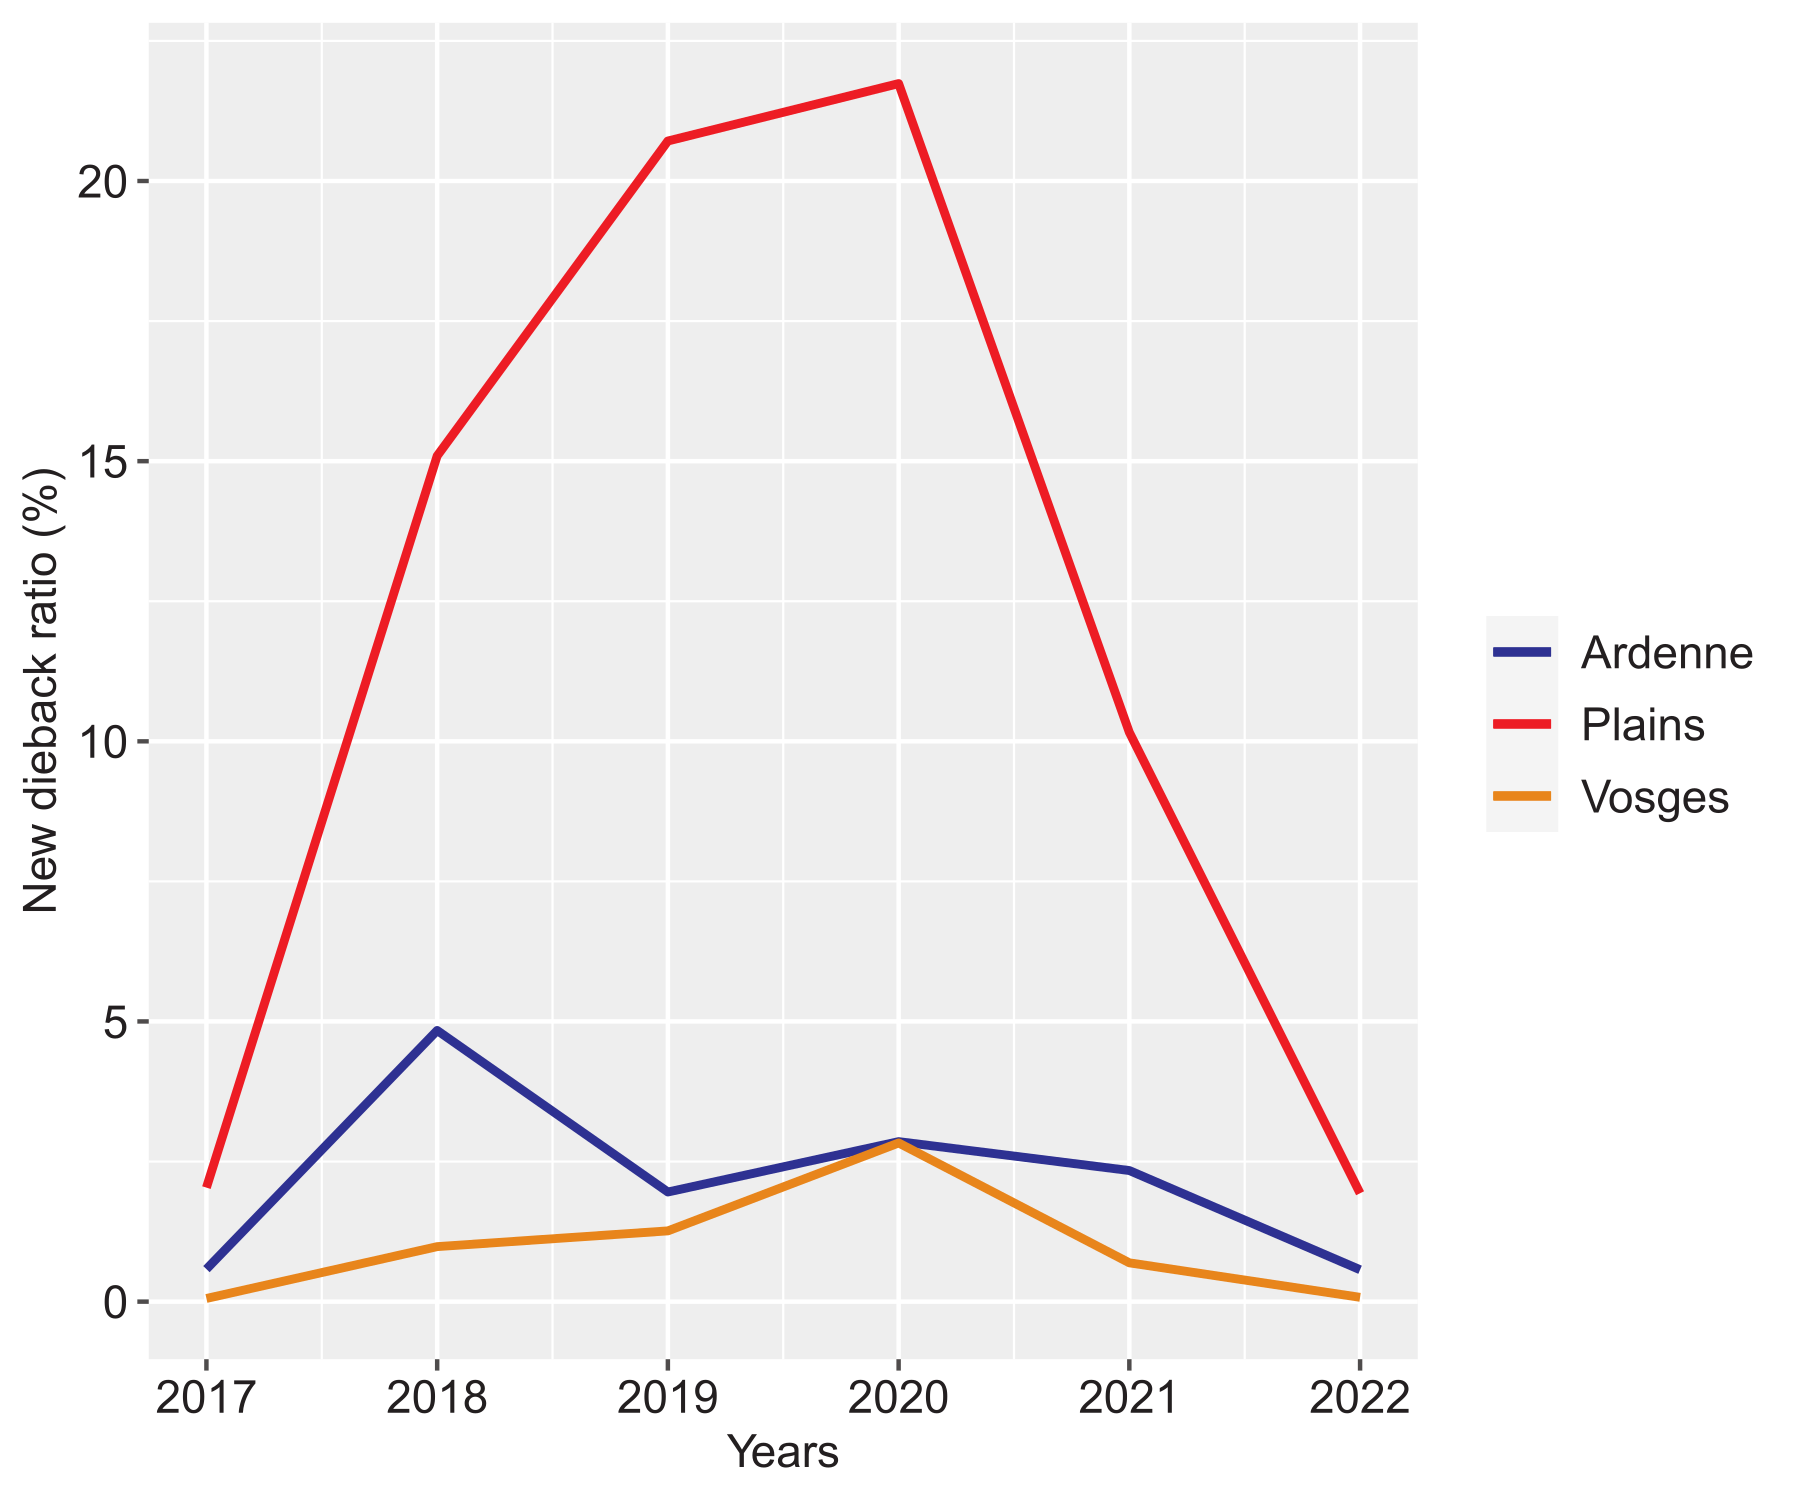
\includegraphics[width=0.6 \textwidth]{Annual_evol_Ardennes_vosges_plaines.png}
    \caption{Proportion of Norway spruce area affected each year  by bark beetle.}
    \label{evol_gen}
\end{figure}

    
\subsection{ Influence of altitude on the Norway spruce mortality}
Because spruce was planted outside its distribution range in low altitude and according to studies showing a shift of species distribution along the altitudinal gradient \citep{lenoir_significant_2008}, more mortality was expected at lower altitude. 
The variation of the dieback rate during 2017-2021  for the three bioclimatic regions.
\begin{figure}[htbp] 
\centering
	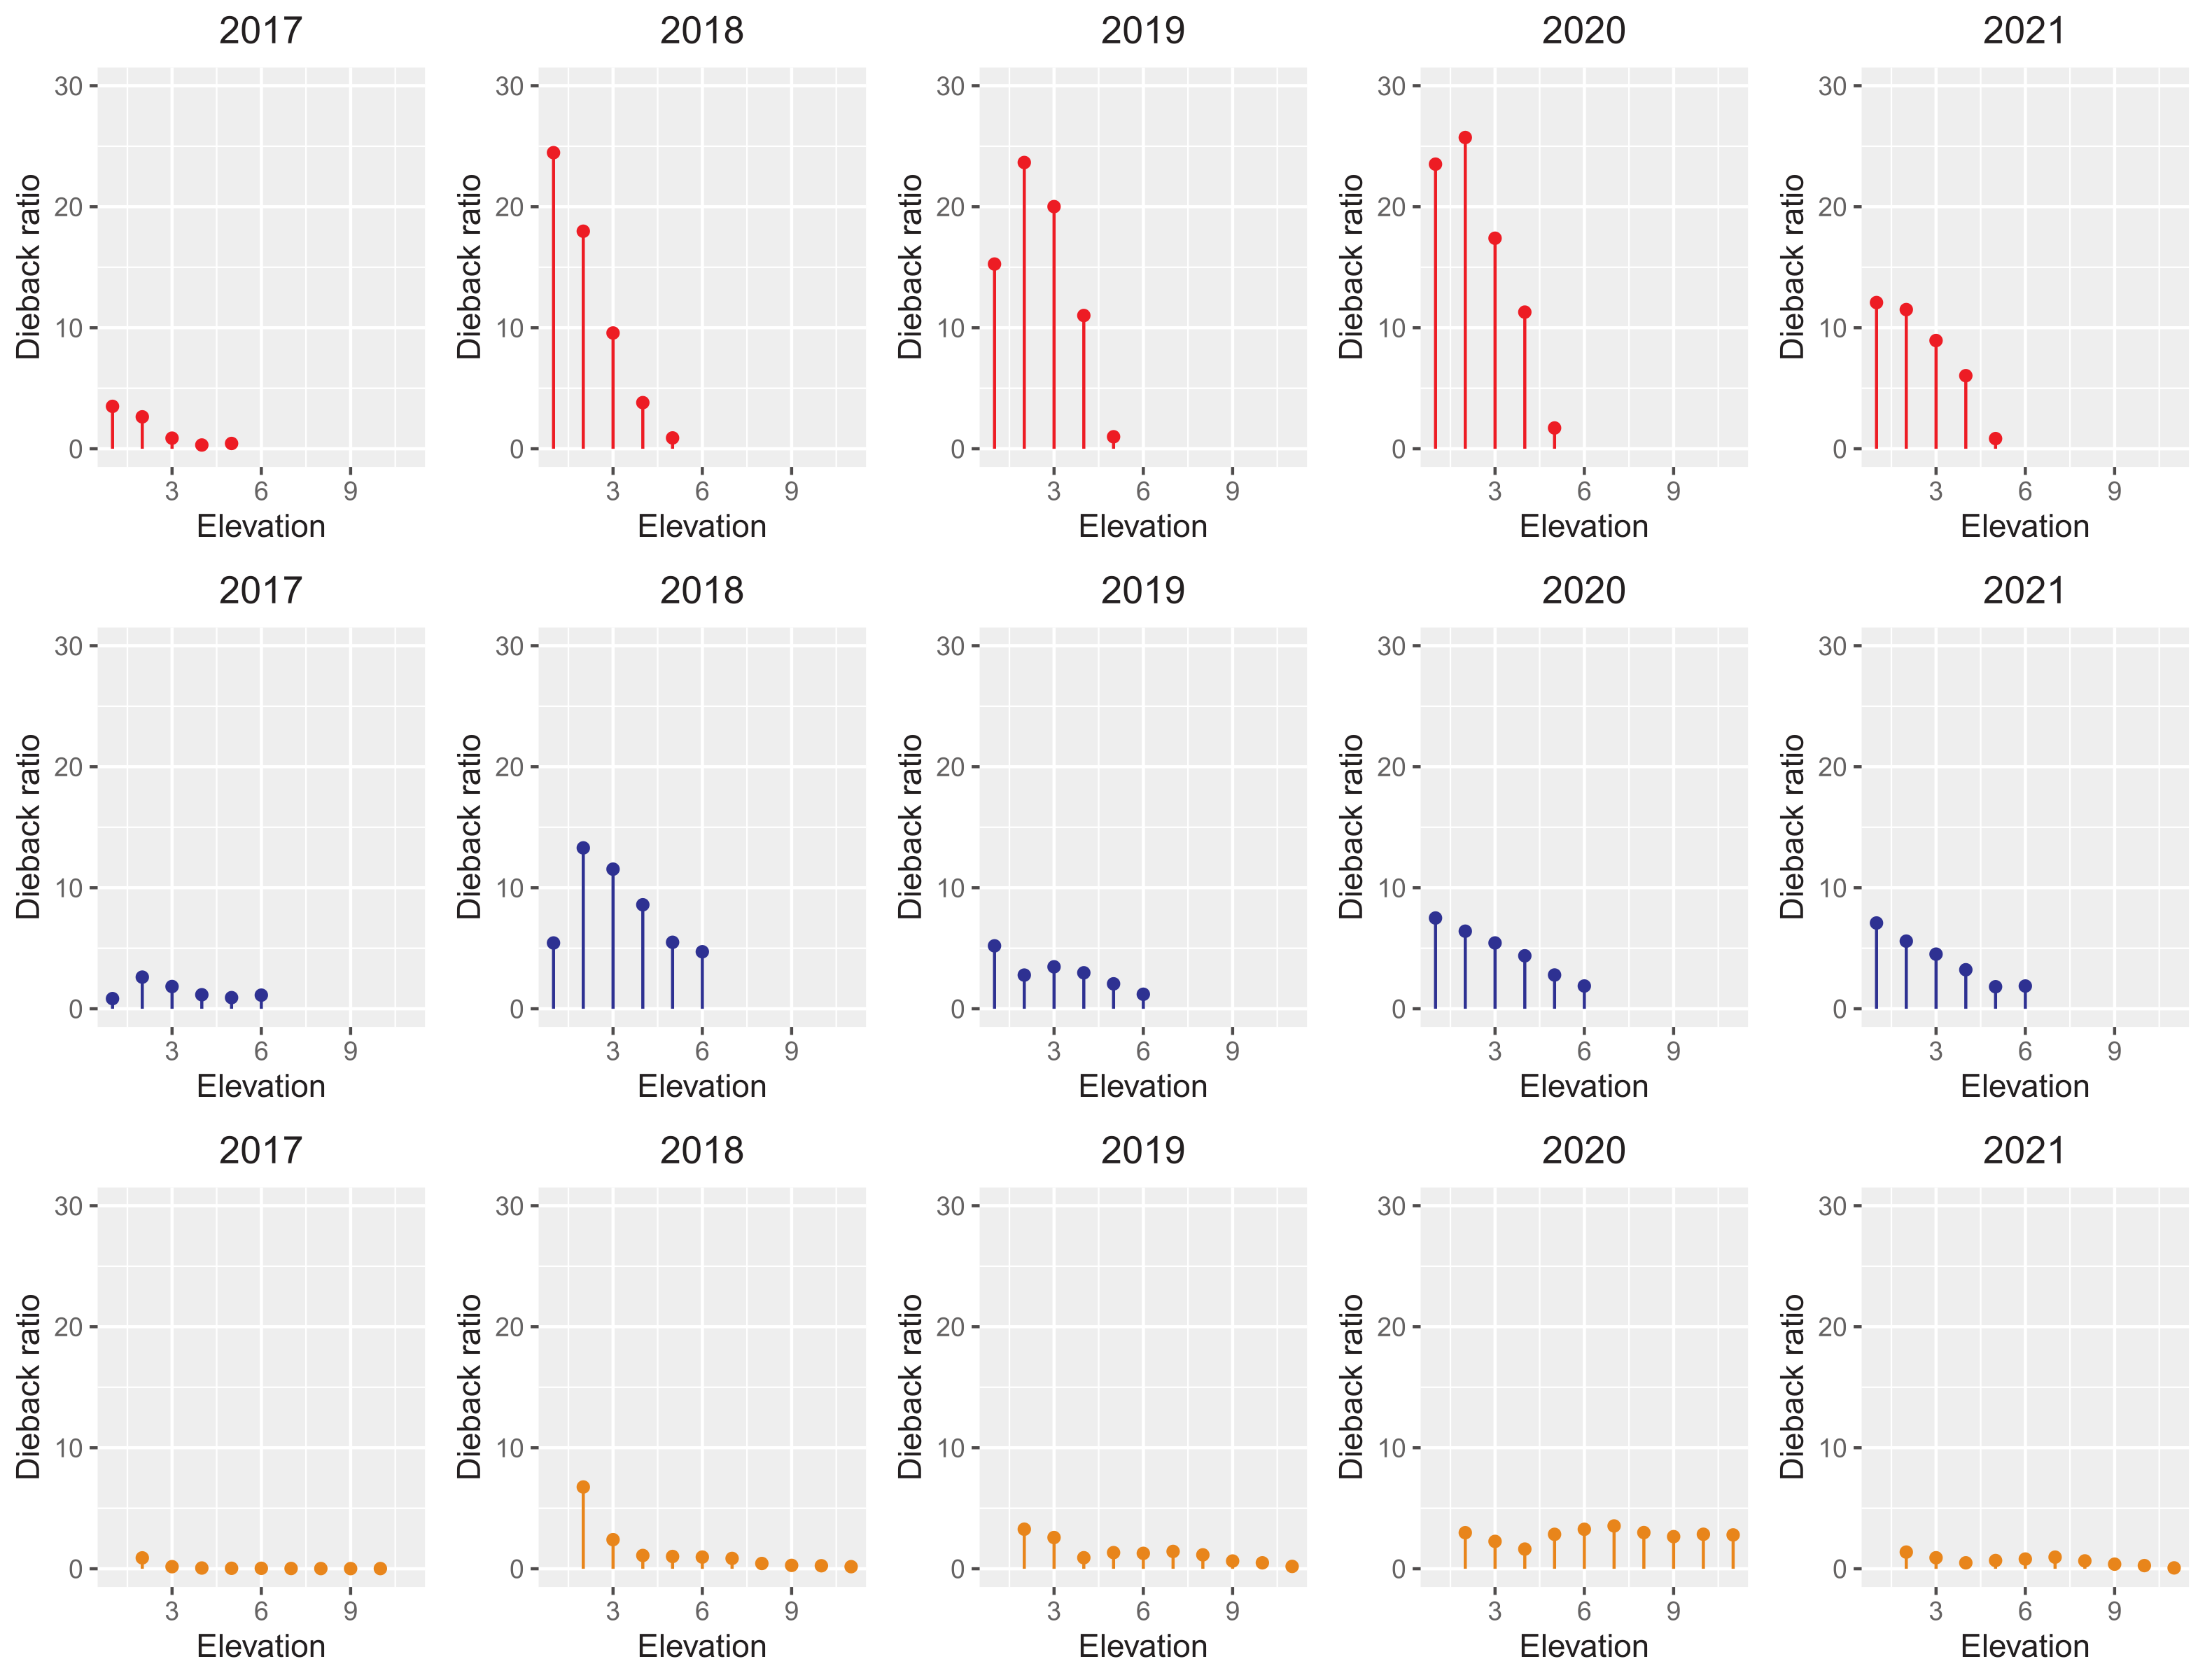
\includegraphics[width=\textwidth]{synthese_color_11_2022.png}
     \caption{Variation of the dieback rate from 2017 to 2022 according to the altitude which has been subdivided into 11 altitude classes of 100 m amplitude for the three regions: Plains (red), Ardenne (blue) and Vosges (orange). 
}
	\label{alti_sco}
\end{figure}
shows an important effect of altitude but with some difference accordinf to the region. More dieback was observed at low altitude :  at the height of the crisis, the probability of new dieback exceeded 20\% each year in the altitude class under 300 m.
In Ardenne, since the beginning of the crisis, the dieback rate is gradually decreasing when altitude is increasing.
Except during 2018, at the peak of the crisis, spruce forest above 500 m were not severely affected.
In the Vosges, the dieback rate is globally low during the crisis comparatively to the other regions, except for 2020.
No clear trend seems to emerge according to the altitude except in the beginning of the crisis in 2018 in the lower stands below 400 m altitude.
However,Vosgian spruces are rare below 400 m.



%The decrease the probabilty of bark beetle presence follow an altitudinal gradient.
%The higher the norway spruce stand grows at an altitude, the lower the probabilty of bark beetle presence. 
%For the Grand-Est region, there is an increase in the probability of bark beetle presence between 2019 and 2021. 

%In the Grand-Est stand, the situation differs than is neighbour region. In 2017, there is low presence of bark beetle  at all altitude.
%The crisis begin weakly in 2018 with attack at low altitude.
%However the probability of presence of bark beetle increase until 2020 to reach more than 20\% of norway spruce killed at altitude below 300m.
%Above 400m, the decreasing didn't follow a altitudinal gradient.
%The probability of presence of bark beetle is relatively constant with a little increase between 700-800m.
%Above 400m, the altitude didn't protect spruce against bark beetle attack in the Grand-Est.

%Unlike the Walloon spruce forest, there is no clear altitudinal gradient in the Vosges. 
%As in Wallonia, the 200-300m altitude class is strongly affected by the bark beetle. The probability of presence decreases along an altitudinal gradient between the altitude classes 200-300 and 400-500m. However, above 500m the probability of bark beetle increases up to the altitude class 700-800m.
%_Description figure \ref{fig:sco_alti} 
% augmentation de la probabilité de présence jusqu'en 2020 et diminution en 2021
% Wallonie: Diminution de la probabilité de présence de scolyte avec l'augmentation de l'altitude 
% Vosges pas de relation clair avec l'altitude. Cependant, les classes d'altitude 2, 11 et 12 semblent + touchées que les autres classes d'altitude
% et ne pas oubnlier de citer untel et machin
	
% Wallonie + Vosges: Augmentation de la probabilité de présence de scolyte avec le temps quelque soit la classe d'altitude.


\subsection{Influence of  exposures on the Norway spruce mortality.}
The cumulative killed areas of Norway spruce during five years of crisis according to the exposures is presented in the table \ref{tab_or_topo} and shows contrasted results according to the region. 
For plains, the north-facing slopes are significantly but slightly more  affected than the plateaus or the south-facing slopes.
In Ardenne, the plateaus are significantly less impacted than the north and south facing slopes. 
In this region, the south-facing slopes are significantly more affected. 
As opposed to the Ardenne, in the Vosges, the plateaus are significantly more impacted than the north and south-facing slopes.
\begin{table}[htbp]
\caption{Par of the studied area killed by bark beetle according to the exposures during the 2017-2022 period.
The same letters (a, b, c) identify homogenous groups with no significant differences for each exposures  (based on  Pearson's chi-squared test statistic, p-value $< 0.05$)}
\label{tab_or_topo}

\begin{tabular}{|l|lll|}
\hline
\multirow{2}{*}{}  & \multicolumn{3}{l|}{Dieback rate (\%)}                             \\ \cline{2-4} 
                   & \multicolumn{1}{l|}{Plains} & \multicolumn{1}{l|}{Ardenne} & Vosges \\ \hline
Plateau            & \multicolumn{1}{l|}{$51.8^a$ }    & \multicolumn{1}{l|}{$11.9^a$}    & $7.2^a$   \\ \hline
South-facing slopes & \multicolumn{1}{l|}{$51.5^a$}   & \multicolumn{1}{l|}{$15.2^b$}    & $5.4^b$    \\ \hline
North-facing slopes & \multicolumn{1}{l|}{$54^b$}   & \multicolumn{1}{l|}{$14.4^c$}    & $5.1^c$   \\ \hline
\end{tabular}
\end{table}

  %rajouter les effectif des pentes et des plateau 

\section{Discussion}

\subsection{Potential methodological limitations}
The detection of dieback is based on dense time serie of Sentinel 2 satellite imagery. \\
The sanitary map uses a species composition map that depend of the spectral response of the vegetation.
In pure even-aged Norway spruce stand, the spectral response is stable in absence of mortality but at edge of this stand and in mixed stand, this response can vary with season due to the deciduous tree or herbaceous species.
In mixed forest and in the border of the stands, the species composition map is less accurate than in pure even aged stand.
In Ardenne and in the Plains, Norway spruce occurs principally in pure even-aged stands of  but in the Vosges forests are more finely mixed.
The annual dieback rate is influenced by Norway spruce area of the composition map.
In Ardenne and in the Plains, the area is correctly estimated.
However, in the mixed stands of the  Vosges, the area is more difficult to evaluate.
An underestimation of dieback rate is not excluded.
Another limitation of the methodology is linked to the felled trees.
To limit the damage of bark beetles, it is recommended to quickly remove the attacked trees from the forest.
However, if the trees are felled before three images are taken by the satellite, the area will be considered as cutted for normal harvesting  rather than for a sanitary thinning.
On the contrary, some felled trees of sanitary thinnings can be healthy but considered as attacked.   
 
\subsection{Dynamic of the dieback}
In forest, sanitary crisis lasts on average between three and ten years \citep{brunier_guide_2020}.
In our study, the spruce dieback have begun in 2018 and decrease in 2022 in all the regions.
The annual dieback rate has recover in the 2022 the same level than in 2017.
The Plains bioclimatic region is the most impacted region.
Since the first year of the study, the new dieback rate has increased until it reached its peak in 2020.
In the Ardenne, the peak were reached directly in 2018 during the first drought period.
A decrease of the dieback occurred during the year 2019.
After the peak the dieback rate has stabilised below 3 \%.
The Vosges were the less impacted bioclimatic area. 
The peak of the crisis was reached in 2020 with 2.8 \% of affected spruce.
During the five years of the crisis, the new dieback rate remained below 3 \%.


\subsection{Regional impact of the bark beetle attacks}
The  impact of the bark beetle attacks is different between the three main regions.
It could be explained through three parameters which differentiate them : the climate, the stand structure and composition, and the current spruce forest management.
Warm and dry climate, as in the Plains, does not meet the autecological requirements of the spruce species, especially during extreme dry or warm events as in the period 2018-2020 \citep{rousi_accelerated_2022} which stressed the spruce. Moreover during warm seasons, the bark beetle produce multiple generations in a year \citep{annila_influence_1969,baier_phenipscomprehensive_2007} that can easily attack these stressed trees.
At the other hand, pure even-aged spruce stands of the Plains and Ardenne are significantly more sensible to pests attacks \citep{faccoli_composition_2014,jactel_2021} than the spruce trees beneficing from continuous cover forestry in mixed stands of the native forest in the Vosges mountains.
Rapid harvesting of trees attacked by bark beetles protects stands from severe outbreaks \citep{stadelmann_effects_2013} but this operation is not systematic in region such as Plains where softwood forestry is not part of the tradition and is not supported by local industry.
Faced with these three parameters, the three main regions are not equal.
In the Vosges, all parameters are favourable, which could explain the limited outbreak during the crisis (5.7\% of initial area).
Indeed, on the opposite, in the Plains all parameters are unfavourable : the warm and dry climate stressed the trees and favoured the beetles which produced large outbreaks in even-aged pure stands, probably less concerned by sanitary thinning. 
These conditions explain that the outbreak was not controlled and reached 52 \% of the spruce area.
The Ardenne spruce forest is an intermediate situation.
The climate is the coldest of the three bioclimatic areas, but less humid then the Vosges.
The forest manager generally make the necessary sanitary felling which is part of the silvicultural tradition.
However, spruce grows in pure even-aged stands.
These conditions could explain an intermediate situation with damages on 12.2 \% of the spruce initial area.


\subsection{Influence of the topographical exposures on the dieback of Norway spruce.}

%citer auteur versant sud + touché
The exposure  influences received radiation and water balance.
South facing slopes are warmer than north facing ones. %reference
As the life cycle of the bark beetle is influenced by temperature \citep{baier_phenipscomprehensive_2007},
this insect should produce more generations in south-facing slopes and thus cause  more damage in this exposure \citep{jakus_1995}.
Moreover, there is 50 \% less water reserve in south-facing slopes than in north-facing slopes in spring \citep{Rouse_1969}.
Thus, Norway spruces that growth in this orientation should be more often in a situation of water stress and should be more attacked than the north-facing slopes.
However, our results do not  clearly fit with this hypothesis. In the Plains, the south-facing slopes and the plateaus are more or less attacked at the same way than the north-facing slopes. In Europe and in north America, Gazol \citep{gazol_2017} observed that species that grow in drier condition area are more resilient to drought.
Piedallu \citep{piedallu_spatial_2022} confirmed this observation in the Vosges during the last outbreak.
Moreover in France, a recent study of \cite{nardi_drought_2022} showed that Norway spruce stand on the steep slopes and soils with low water availability are less attacked.
In this Vosges, spruce trees growing on the southern slopes and plains have suffered of drier conditions throughout their lives and therefore have been less stressed than spruce trees growing on the north-facing slopes.
In Ardenne, the south-facing slopes are more affected by bark beetle than other position.
Norway spruce that growth in south-facing slopes should be more often in a situation of water stress and should be more attacked than the north facing-slopes.
However the north-facing slopes are not the less attacked. 
The shallow soil depth on the slopes could explain the dieback rate difference between de slope and the plateaus. 
In the Ardenne and in the Vosges, the result are opposed for the plateaus.
The damage caused in the Vosges plateaus could be explained by the more important presence of pure even-aged stand in this topographical orientation than in the slope.
This stand structure is more sensible to bark beetles.

The trend of bark beetle attacks following the topographical exposures need further investigations.
In view of these results, it seems difficult to give global advice for forest managers.
\section{Conclusion and perspectives}
Our study aimed to assess the evolution of the bark beetle crisis in the spruce forest with a remote sensing approach.
The methodology used to identify the damaged stands is robust and effective as far as reliable species composition maps are available.
Indeed, to improve the result in the Vosges, a new Norway spruce map is necessary to better distinguish spruce from fir.
Taking this limitation into account, remote sensing could be the basis for monitoring bark beetle attacks in spruce forest.
This crisis triggered by the dry and warm events from 2018 to 2020 lasted five years and destroyed 14 \% (29.000 ha) of the spruce area in Wallonia and Grand-Est of France.
In 2022, new bark beetle attacks recover its level of 2017 and seems then over.
The damages were not equally distributed on the territory : the Plains are the most impacted regions with more than 50\% of the spruce area impacted by bark beetles.
The devastated area by this pest is estimated around 11,000 ha.
The Ardenne is the second region that has lost the most spruce area with  12,4 \% of his spruce area attacked or around 13,400 ha. 
The Vosges is the less attacked region with 5.7 \% of his spruce area killed. The total area impacted in this mountain region is around 4,300 ha.
This situation could be linked to the climate, the structure and the composition of the stands, and the current forest monitoring and management which differ between the three regions.
Taking into account the climate change, which will favour warm and dry events in the near future, our results does not support new plantations of Norway spruce in Plains.
In Ardenne, we advise not to plant any more Norway spruce at lower altitude then 400 m except in specific micro-climate.
In the Vosges, the trend differs of the two others regions.
More investigation specially dedicated to this region is necessary to draw conclusions.
A study taking into account the effects of environment, climate and silvicultural factors would be interesting to better understand the determining factors of these bark beetle attacks of this important species for the wood industry.

%The Vosges climatic area is the less impacted by the dieback and the Plains the most affe
%Dans des régions très proches, les stations de dépérissement de l'épicéa sont différentes.
%Il semble donc difficle de généraliser des modèles basé sur des relations topographique à une grande échelle.


	

%\begin{figure}[htbp]
%	\begin{minipage}[b]{1 \linewidth}
%		\centering
	%	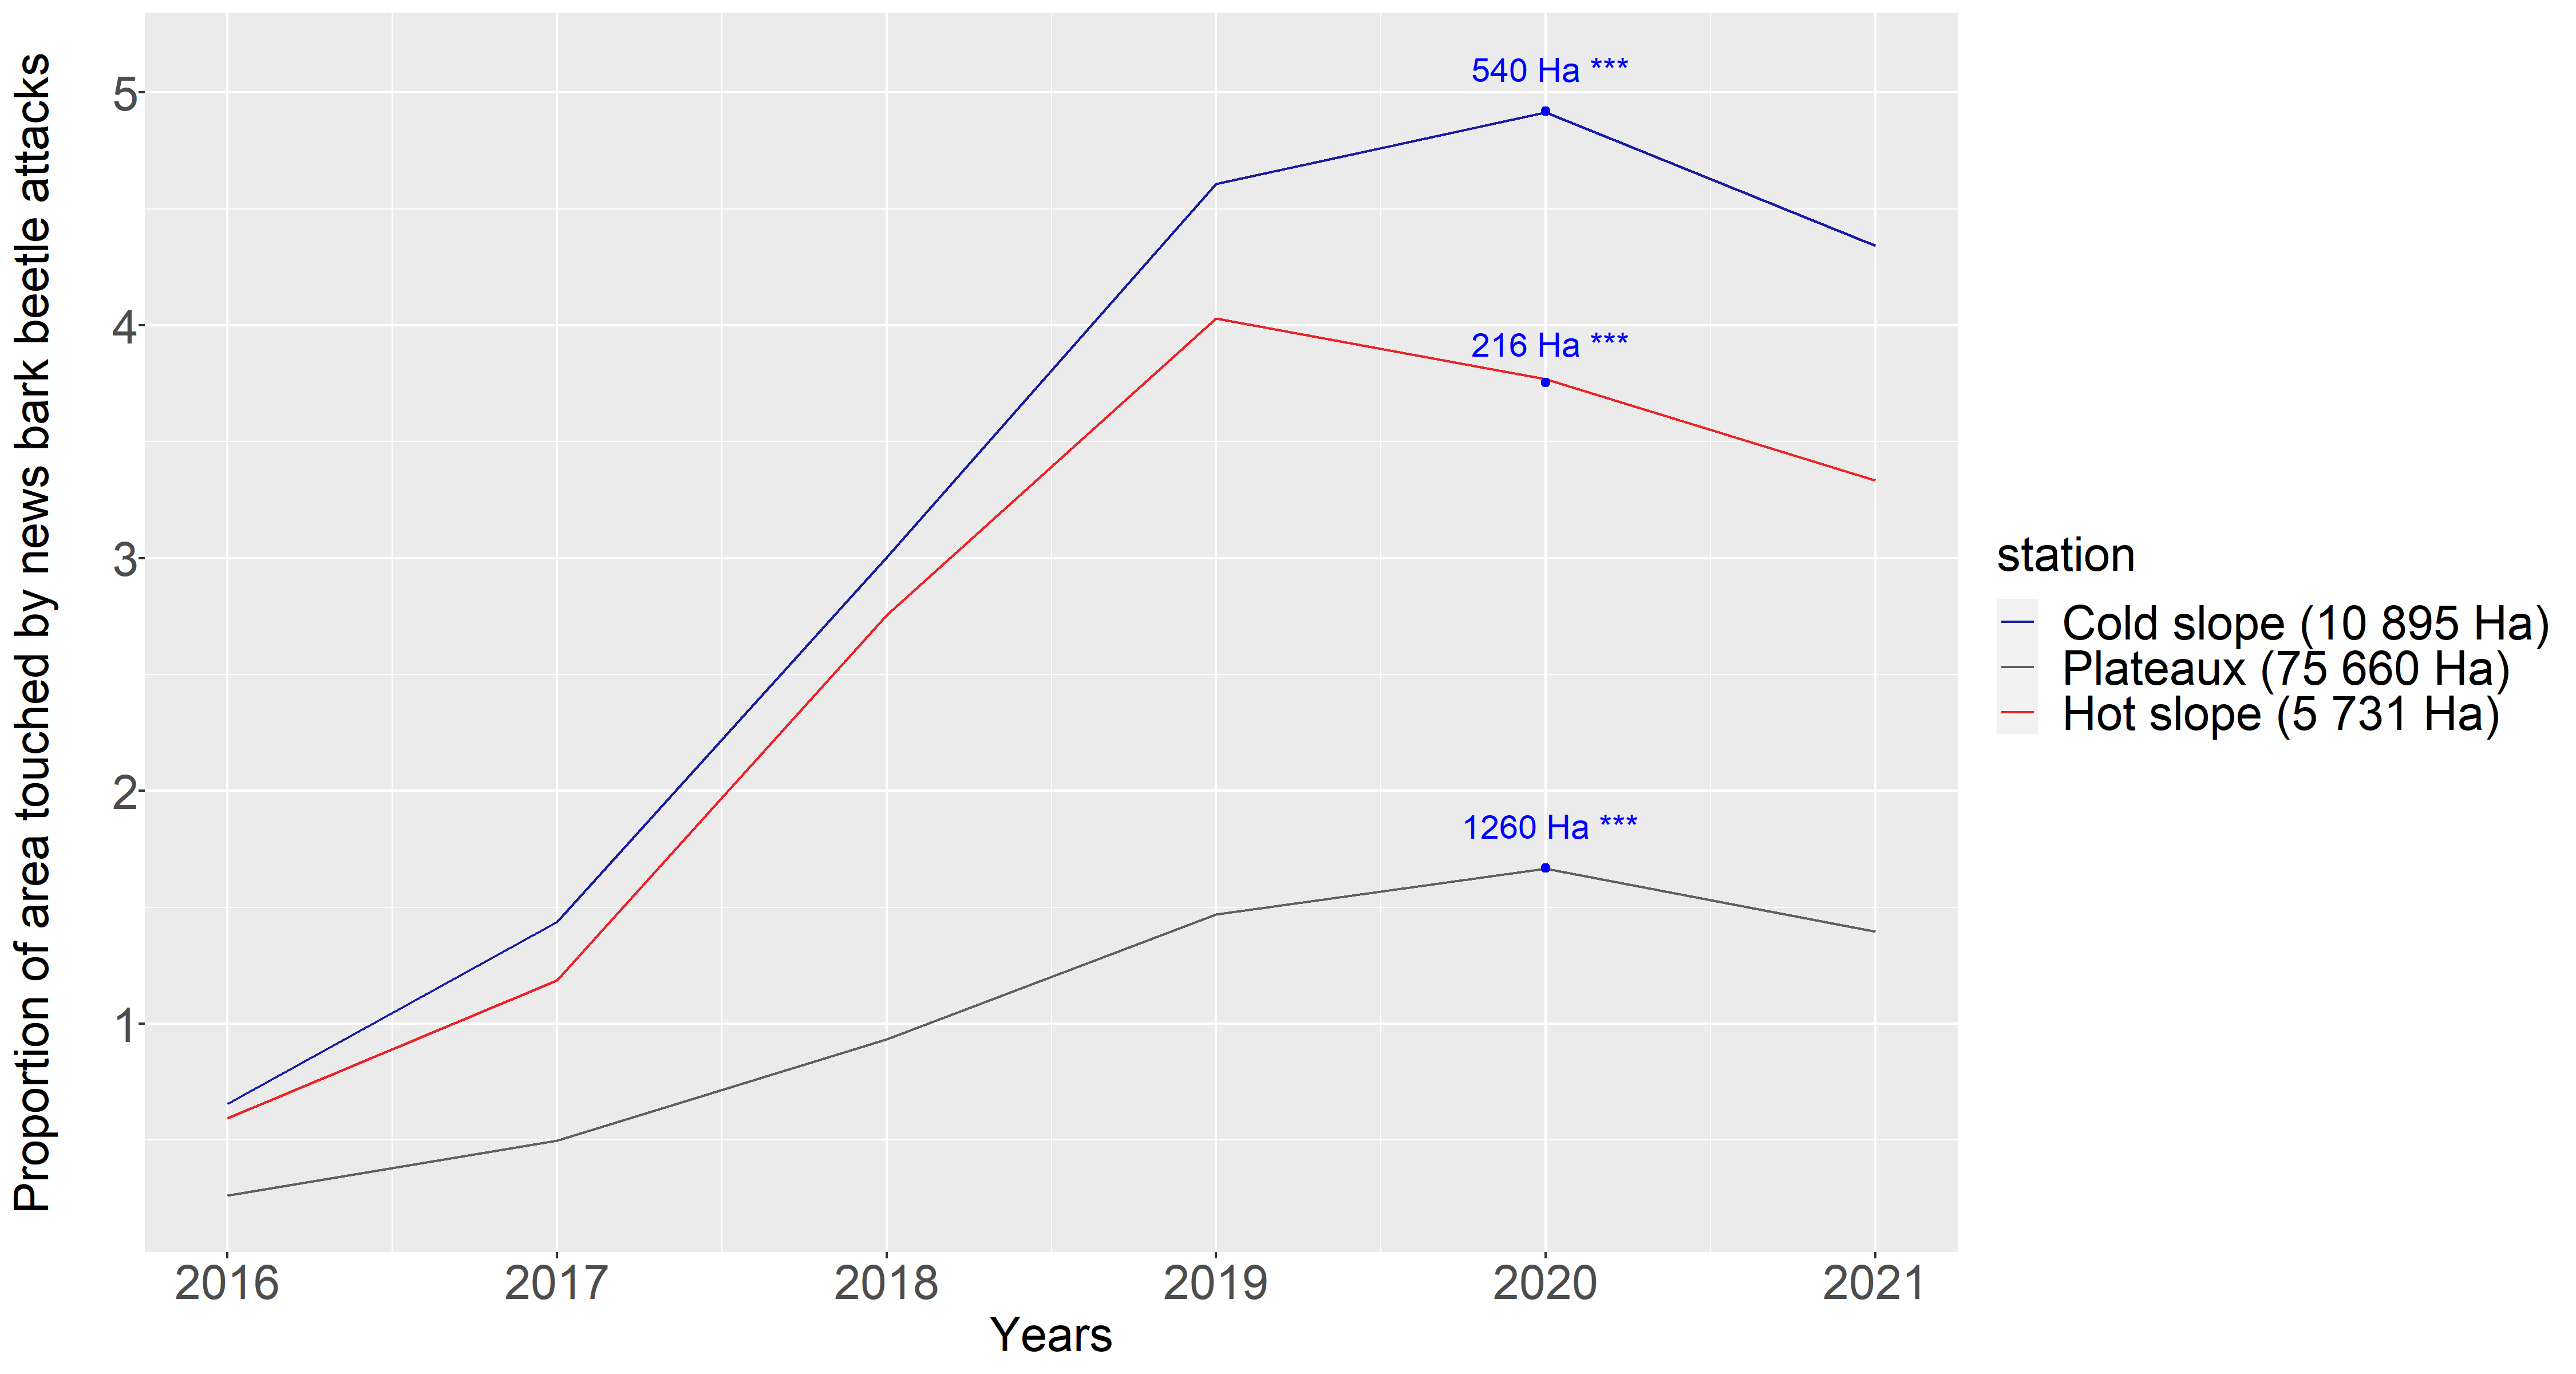
\includegraphics[width=1\textwidth]{evol_ss_wal.png}
%		\caption{Évolution de la crise du typographe en région wallonne en fonction des sous-secteurs.}
%		\label{fig:ss_wall}
		%\caption sert à insérer une légende
%	\end{minipage}\hfill
%	\vspace{1cm}
%	\begin{minipage}[b]{1 \linewidth}
%		\centering
%		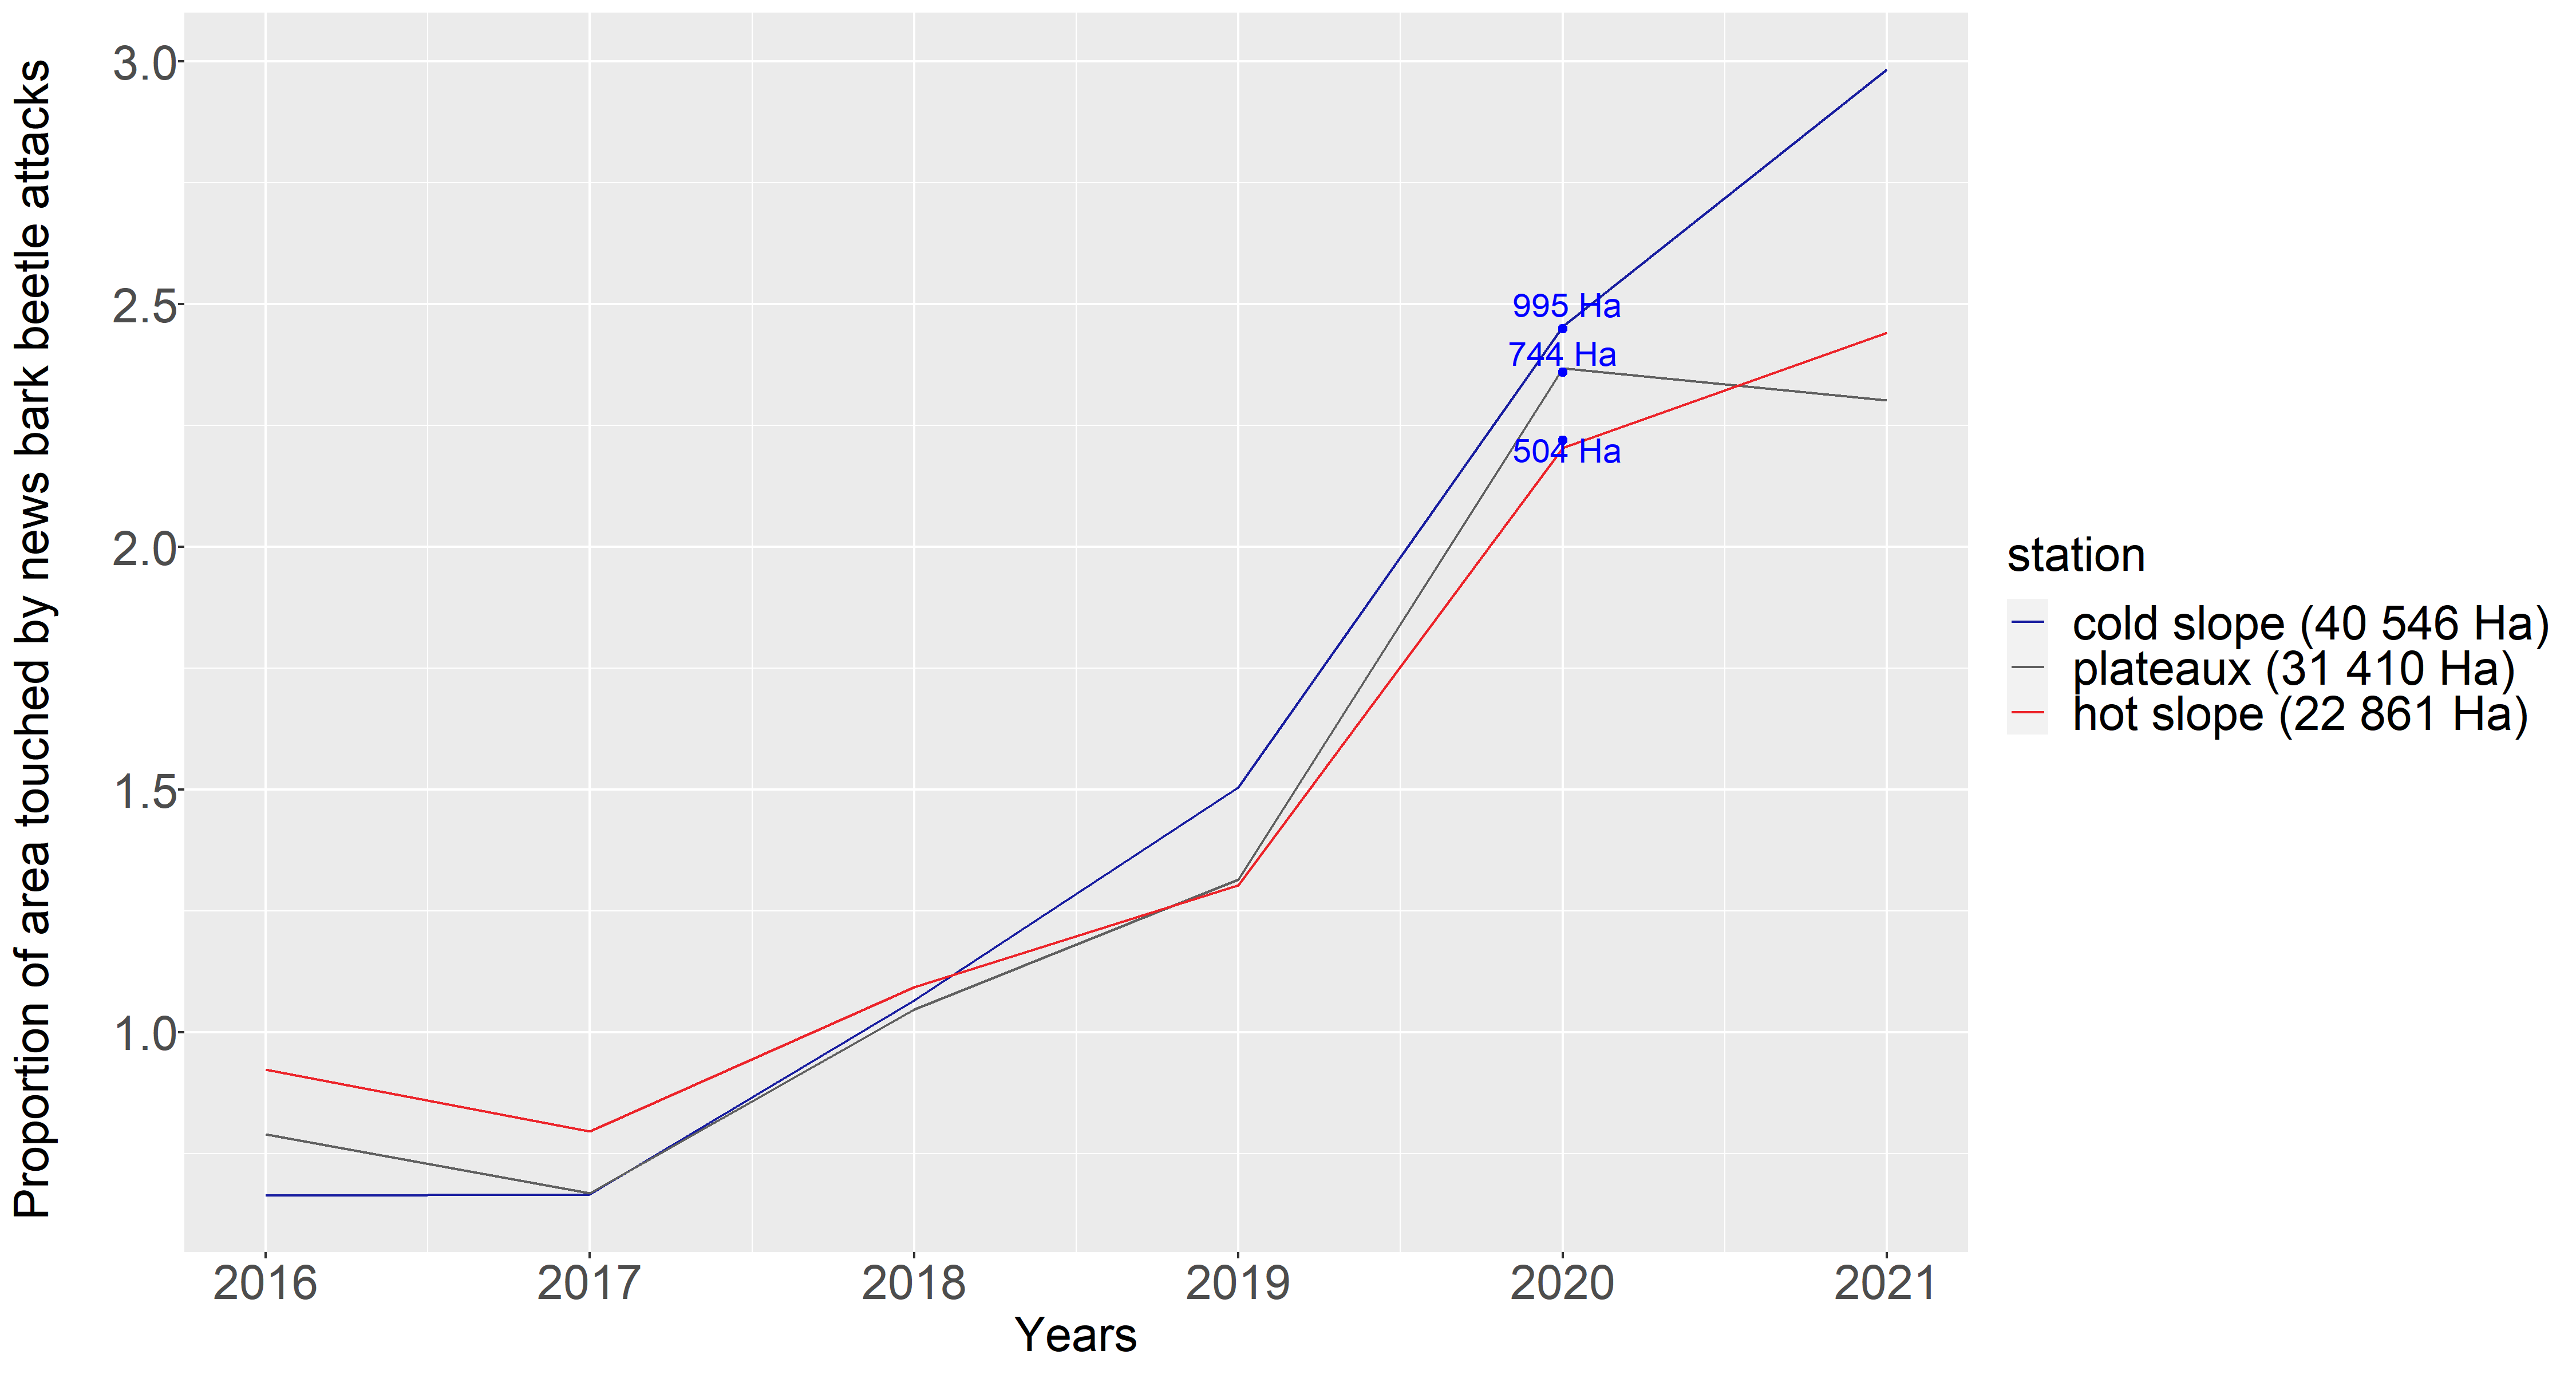
\includegraphics[width=1\textwidth]{evol_ss_vosges.png}
%		\caption{Évolution de la crise du typographe dans les Vosges en fonction des sous-secteurs .}
%		\label{fig:ss_vosg}
%	\end{minipage}
%end{figure}

\section{Acknowledgements}

This research has been funded thanks to the \textit{RegioWood II} project and to the \textit{Plan quinquennal de recherches forestières} of the Service Public de Wallonie (forest administration).

%\bibliographystyle{elsarticle-num}
\bibliographystyle{plainnatGL_v2}\biboptions{authoryear}
\bibliography{Scolyte.bib}
\end{document}
